\documentclass[12pt]{extarticle}
\usepackage[utf8]{inputenc}
\usepackage{mathtools}
\usepackage{amsthm}
\usepackage{amsfonts}
\usepackage{tikz}
\usepackage{tkz-berge}
\usepackage{hyperref}
\usepackage{float}
\usepackage[ruled,vlined]{algorithm2e}
\usepackage{todonotes}

\theoremstyle{definition}
\newtheorem{definition}{Definition}
\theoremstyle{remark}
\newtheorem{note}{Note}
\theoremstyle{plain}
\newtheorem{theorem}{Theorem}

\newcommand{\BO}{\mathcal{O}}

\title{AuW Recap}
\author{
    Axel Montini
    \\
    \href{mailto:amontini@student.ethz.ch}{amontini@student.ethz.ch}
}

\begin{document}
\maketitle

Cannot be used during the exam, but it's a nice short recap of everything done in the second semester.

\section{Last semester}
Go read again about MST algorithms and so on.

\section{Graphentheorie}

\subsection{Zusammenhang}
\begin{definition}
    A graph $G=(V,E)$ is \textit{k-zusammenhängend} if $|V| \ge k + 1$ and
    for all $X \subseteq V,\ |X| < k$ the following is true:
    \[ \mbox{The graph}\ G[V \setminus X]\ \mbox{is zusammengehängend} \]
\end{definition}

\begin{definition}
    A graph $G=(V,E)$ is \textit{k-kanten-zusammenhängend} if
    for all $X \subseteq E,\ |X| < k$ the following is true:
    \[ \mbox{The graph}\ G(V, E \setminus X)\ \mbox{is zusammengehängend} \]
\end{definition}

\begin{note}
    A graph can be both 2-kanten-zusammengehängend and be only 1-zusammengehängend at the same time.
    Example:
    \begin{figure}[H]
        \centering

        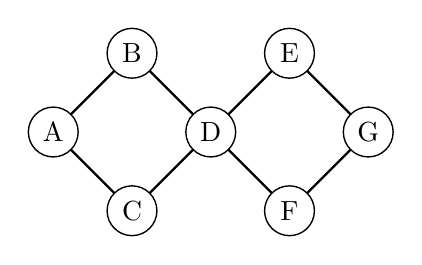
\begin{tikzpicture}
            \Vertex[x=0,y=0]{A}
            \Vertex[x=1,y=1]{B}
            \Vertex[x=1,y=-1]{C}
            \Vertex[x=2,y=0]{D}
            \Vertex[x=3,y=1]{E}
            \Vertex[x=3,y=-1]{F}
            \Vertex[x=4,y=0]{G}

            \Edges(A, B)
            \Edges(A, C)
            \Edges(C, D)
            \Edges(B, D)
            \Edges(D, E)
            \Edges(D, F)
            \Edges(E, G)
            \Edges(F, G)
        \end{tikzpicture}
    \end{figure}
\end{note}

\begin{definition}
    In a zusammengehängend Graph,
    \textit{Artikulationsknoten} disconnect the graph when removed.
    Only 1-zusammengehängend graphs can have Artikulationsknoten
\end{definition}

\begin{theorem}
    In zusammenhängende Graphs it's possible to find Artikulationsknoten in $\BO(|E|)$ if an adjacency list is used.
\end{theorem}

\begin{definition}
    A zusammenhängend Graph may contain \textit{Brücke}. In this case, it's \textbf{not 2-kanten-zusammenhängend}.

    An edge is a bridge if it disconnects the graph when removed.
\end{definition}

\begin{theorem}
    Brücke can also be computed in $\BO(|E|)$ using an adjacency list.
\end{theorem}

\begin{definition}
    $G = (V,E)$ is zusammenhängend. For $e,f \in E$ we define the relation
    \[ e \sim f \Leftrightarrow e = f\ \mbox{or there is a Kreis containing both edges} \]

    This is an equivalence relation. Each equivalence class is called a \text{Block} (plural \text{Blöcke}).
\end{definition}

\subsection{Kreise}

\begin{definition}
    An \textit{Eulertour} in a graph $G$ is a closed path (\textit{Zyklus}) that contains every edge $\in E$ exactly once.

    A graph containing an Eulertour is called \textit{eulersch}.
\end{definition}

\begin{definition}

\end{definition}

\begin{theorem}
    \[ \mbox{A graph is eulersch} \Leftrightarrow deg(v)\ \mbox{is even for all vertices}\]
\end{theorem}

\begin{theorem}
    In a connected and eulersch Graph it's possible to find an Eulertour in $\BO(|E|)$.
\end{theorem}

\begin{definition}
    A \textit{Hamintonkreis} in $G$ is a cycle that goes through every vertex exaclty once.
    A graph containing an Hamintonkreis is called \textit{hamintonsch}.
\end{definition}

\begin{theorem}
    The algorithm seen in class can find an Hamintonkreis in time $\BO(n^2 \cdot 2^n)$ and memory $\BO(n \cdot 2^n)$, where $n = |V|$.
\end{theorem}

\begin{theorem}
    A bipartite graph $G = (A \uplus B, E)$ cannot contain an Hamintonkreis.
\end{theorem}

\begin{theorem}[Dirac]
    A graph $G$ with $V \ge 3$ in which every vertex has at least $|V|/2$ neighbors is \textit{hamintonsch}.
\end{theorem}

\begin{definition}
    In a complete graph $K_n$ (all vertices are connected together),
    the metric Traveling Salesman Problem consists in finding an
    Hamintonkreis $C$ with minimal cost (distance).
\end{definition}

\begin{definition}
    An $\alpha$-Approximationsalgorithmus of this problem finds an H.kreis $C$ so that
    \[ \sum_{e \in C} l(e) \le \alpha \cdot opt(K_n, l) \]
    Meaning that it finds a solution worse by the optimal solution by a factor $\alpha$.
\end{definition}

\begin{theorem}
    If there's an $\alpha$-Approximationsalgorithmus with $\alpha > 1$ for the TSP with running time $\BO(f(n))$ then there's
    also an algorithm that decides whether a graph with $n$ vertices is hamintonsch in $\BO(f(n))$.
\end{theorem}
\begin{theorem}
    For the metric TSP there's a 2-Approximationsalgorithmus with running time $\BO(n^2)$.
    It find the MST in $\BO(n^2)$ and then uses it to find the H.k.
\end{theorem}

\subsection{Matching}

\begin{definition}
    A set of edges $M \subseteq E$ is called \textit{Matching} in a graph $G$ if
    \[ \forall e,f \in M\ (e \cap f = \emptyset) \]

    \begin{itemize}
        \item A vertex $v$ is said to be \textit{überdeckt} by a matching $M$ if the matching contains an edge containing $v$.
        \item A matching $M$ is called \textit{perfektes Matching} if every vertex is überdeckt (equivalent: $|M| = |V| / 2$).
    \end{itemize}
\end{definition}

\begin{definition}
    A matching $M$ is said to be:
    \begin{itemize}
        \item \textit{inklusionsmaximal} if $M \cup \left\{ e \right\}$ is not a matching for all $e \in E \setminus M$.
        \item \textit{kardinalitätsmaximal} if $|M| \ge |M'|$ for all matchings $M'$ in $G$.
    \end{itemize}

    Note that \textit{kardinalitätsmaximal} $\Rightarrow$ \textit{inklusionsmaximal} (the opposite might not be true).
\end{definition}

\begin{theorem}
    \begin{algorithm}
        \caption{Greedy-Matching}
        \KwResult{The inklusionsmaximales matching $M$}
        \While{$E \ne \emptyset$}{
            choose an edge $e \in E$\;
            $M \gets M \cup \left\{ e \right\}$\;
            remove $e$ and all incident edges from $G$\;
        }
    \end{algorithm}

    The greedy-matching algorithm finds an inklusionsmaximal Matching in time $\BO(|E|)$
    for which the following holds: $|M_{Greedy}| \ge \frac{1}{2} |M_{max}|$, where $M_{max}$ is a kardinalitätsmaximales Matching.
\end{theorem}

\begin{theorem}[Berge]
    Let $M$ be a matching in $G$ that is not k.maximal, then there is an augmenting path to $M$.
    \todo{Algos at page 65 and 67}
\end{theorem}

\begin{theorem}
    Is $n$ even $K_n$ a complete graph, then it's possible to find a \textit{minimal perkeftes Matching} in time $\BO(n^3)$
\end{theorem}

\begin{theorem}
    There's a 3/2-Approximationsalgorithmus for the TSP that runs in $\BO(n^3)$.
\end{theorem}

\begin{definition}
    \textit{Nachbarnschaft einer Knotenmenge} $X \subseteq V$:
    \[ N(X) := \bigcup_{v \in X} N(v) \]
\end{definition}

\begin{theorem}[Hall, Heiratssatz]
    For a bipartite graph $G = (A \uplus B, E)$ theres a matching $M$ with $|M| = |A|$ if and only if $|N(X)| \ge |X|$ for all $X \subseteq A$.
\end{theorem}

\begin{definition}
    A bipartite graph is called \textit{k-regulär} if every vertex has degree $k$.
\end{definition}

\begin{theorem}
    Let $G$ be a k-regular bipartite graph. Then there's $M_1, ..., M_k$ so that $E = M_1 \uplus M_2 \uplus ... \uplus M_k$ and all
    $M_i, 1 \le i \le k$ are perfect matchings.
\end{theorem}

\begin{theorem}
    Is $G = (V, E)$ a $2^k$-regular bipartite Graph, then it's possible to find a perfect matching in $\BO(|E|)$.
\end{theorem}

\subsection{Färbungen}

\begin{definition}
    A \textit{(Knoten)-Färbung} (vertex coloring) of a graph $G$ with $k$ colors is $c: V \to [k]$, so that
    \[ c(u) \ne c(v)\ \forall \left\{ u, v \right\} \in E \]

    The \textit{chromatische Zahl} (chromatic number) $X(G)$ of a graph is the minimal amount of colors that can be used to
    color $G$.
\end{definition}

\begin{theorem}
    A graph is bipartite if and only if doesn't contain any Kreis of odd length.
\end{theorem}

\begin{theorem}[Vierfarbensatz]
    Every map can be colored with 4 colors.
\end{theorem}

\begin{theorem}
    \begin{algorithm}
        \caption{Greedy-Färbung}
        \KwData{$G$}
        \KwResult{array $c$ mapping each vertex to a color}
        $c(v_1) \gets 1$\;
        \For{$i = 2, \dots, n$}{
            $c(v_i) \gets \min \left\{ k \in \mathbb{N} \mid k \ne c(u)\ \mbox{for all}\ u \in N(v_i) \cap \left\{ v_1, ..., v_{i - 1} \right\} \right\}$
        }
    \end{algorithm}

    Let $G$ be a connected graph and $C(G)$ the amount of colors used by the Greedy-Färbung algorithm.
    Then
    \[ \mathcal{X}(G) \le C(G) \le \Delta(G) + 1 \]
    Where $\Delta(G) := \max_{v \in V} deg(v)$ is the max degree in the graph.

    The running time is $\BO(|E|)$ if an adjacency list is used.
\end{theorem}

\begin{theorem}[Brooks]
    Let $G$ be a connected graph that is neither complete nor an odd Kreis ($G \ne K_n$ and $G \ne C_{2n+1}$).
    Then
    \[ \mathcal{X}(G) \le \Delta(G) \]
    And there's an algorithm that can color the vertices of $G$ in time $\BO(|E|)$ and with $\Delta(G)$ colors.
\end{theorem}

\begin{theorem}[Mycielski-Konstruktion]
    For all $k \ge 2$ there's a triangle-free graph $G_k$ with $\mathcal{X}(G) \ge k$.
\end{theorem}

\begin{theorem}
    Every 3-färbbaren graph can be colored in time $\BO(|E|)$ with $\BO(\sqrt{|V|})$ colors.
\end{theorem}

\section{Randomized algorithms}

\end{document}
